\chapter{Reinforcement Learning}
Machine learning consists of three approaches to problem-solving: Supervised learning, unsupervised learning and
reinforcement learning.
We will focus on the latter one, as reinforcement learning enables agents to learn complex behaviour through
exploration within an game environment.
In this chapter I will briefly explain the key concepts and methods of reinforcement learning that allow our model
learn the game of Schafkopf.
For this we will explain neural networks, their components and internal mechanisms, the reinforcement learning approach,
Proximal Policy Optimisation, which is the training algorithm used in our experiments, and Actor-Critic models.

\section{Neural Networks}
A \textbf{Neural Network (NN)} is an attempt to imitate the complex behaviour of the human brain that
enables us as humans to learn complex skills.
The human brain consists of billions of neurons, the basic building block inside the nervous system, that are
interconnected to form large networks, capable of processing an input signal,for example a visual stimulus, into an
output.\\

\subsection{Artificial Neuron}
To imitate this we define an artificial neuron, with the goal of creating a type of switch to process an input signal
to an output, which could again be connected to further neuron.
To do so, we give the artificial neuron an input, a weight associated with that input,an activation function and an
output.
A neuron may have multiple inputs as well as outputs and the connection between the output of one neuron to the input
of another neuron is called an edge, which in turn may have their own weights.
The output signal is calculated by passing the sum of all weighted input signals through the activation function and
can be express by the following formula:
\newline
\begin{center}
    \begin{math}
        \boxed{
            \begin{aligned}
                &\textrm{Let } k\textrm{ be the neuron }k,&\\
                &\textrm{let } n \textrm{ be the number of inputs }x,&\\
                &\textrm{let } w \textrm{ be the weight,}&\\
                &\textrm{and let }\phi \textrm{ be the activation function}&\\
                &y\textsubscript{k} = \phi (\sum_{i=0}^n w\textsubscript{kn}x\textsubscript{n})
            \end{aligned}}
        \caption{Formula to calcualate neuron output }
        \label{neuronactivation}
    \end{math}
\end{center}
There are a number of possible activation functions that can be used, but for our purpose we will look at
\textbf{Rectified Linear Unit (RELU)} and the \textbf{Softmax}.\\
\newline
\textbf{ReLU} is a simple activation function that forwards the input, if its positive, otherwise zero.
The \textbf{ReLU} function is formulated using:

\begin{center}
    \begin{math}
        \boxed{
            \begin{aligned}
                &\textrm{Let } x \textrm{ be the input of a \textbf{ReLU}}\\
                &f(x) = max(0,x)
            \end{aligned}
        }
        \caption{Definition of \textbf{ReLU} activation function}
        \label{activationRelu}
    \end{math}
\end{center}
\textbf{ReLU}, when compared to the more tradition Sigmoid activation function, has proven to be favourable in terms
of computational efficiency and performance, when applied to deep neural networks. \cite{krizhevsky2012imagenet}
For this reason we exclusively use \textbf{ReLU} in all input and hidden layers.
\\
\textbf{Softmax} is a useful activation function for output layers, as they transform any input regardless of
absolute size to an output that is within [0,1].
The output of an output layer with \textbf{Softmax} is a normalised probability distribution, where each neuron in
the layer has a probability, and the sum of all probabilities is 1.
The definition of \textbf{Softmax} is the following:
\begin{center}
    \begin{math}
        \boxed{
            \begin{aligned}
                &\textrm{Let } z \textrm{ be the vector of } N \textrm{ inputs} \\
                &f(z)_{i} = \frac{e^{z_{i}}}{\sum_{j=1}^{N} e^{z_{j}} }
            \end{aligned}
        }
        \caption{Definition of the \textbf{Softmax} activation function}
        \label{activationSoftmax}
    \end{math}
\end{center}
\newline
Now that we defined a neuron, we can use multiple neurons to form a layer, which in turn can be connected in sequence
to form a \textbf{NN}.
The minimal architecture of a network consists of three layers, whereas the middle layers are named hidden layers:
\[\text{Input layer}\Rightarrow\text{Hidden layer}\Rightarrow\text{Output layer}\]
\newline
Between adjacent layers, every neuron's input is connected to the outputs of every neuron in the previous layer and
vice versa for the following layer.
See Fig. \ref{fig:architecture} for an example.
\newline

\begin{figure}[h!]
    \centering
    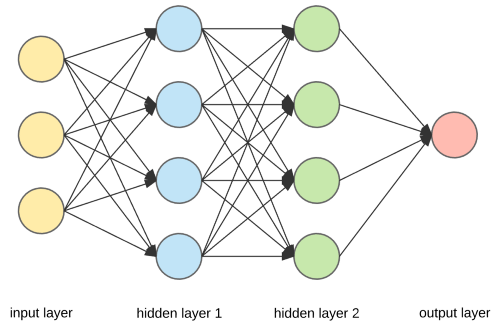
\includegraphics[scale=0.5,]{neuralnetlayer}
    \caption{Example architecture of a neural network with input,2 hidden and output layers}
    \label{fig:architecture}
\end{figure}
This kind of architecture is called \textbf{feed forward NN}, due to the process of passing an input linearly through
the network to the output, and will be used exclusively in our experiments.\\

\subsection{Policy}
The strategy for an agent to use inside an environment is called a \textbf{Policy}($\pi$).\\
The environment in our case is the game of Schafkopf, where an agent receives information about the current game
state(\textit{s}) at the time of his action that, which we use as input in our NN to make a decision on what action
(\textit{a}), in our case an action in the form of a valid card from our hand, to take.
At the end of each a hand we collect a reward(\textit{r}), which our policy over time tries to maximise.\\
We can define our policy as a function that takes a state and returns the probability of an action:\\
\[ \pi(s)\rightarrow P(a)\]\\
Ideally we would want our policy to be optimal, for which we require a method of updating our NN using the
experiences and rewards we gained through interaction with the environment.
By optimal we understand, that from any given state \textit{s\textsubscript{i}} we maximise the reward \textit{r}
For this we use


\section{Actor-Critic}


\section{Proximal Policy Optimisation}


\section{Self Play Learning}
